\documentclass{../exhibit}

\title{Pirate Pizza}

%% Font
\usepackage{imfellEnglish}
\usepackage[T1]{fontenc}
\raggedright

\usepackage{background}

\backgroundsetup{
scale=1,
color=black,
opacity=0.4,
angle=0,
contents={%
  \includegraphics[height=\paperheight]{mapBackground.jpg}%%https://upload.wikimedia.org/wikipedia/commons/8/81/Nautical_chart_of_the_West_Indies_1797.jpg
  }%
}




%% For the context
%% https://tex.stackexchange.com/questions/86150/torn-page-effect/86151#86151
\usepackage{tikz}
\usetikzlibrary{decorations.pathmorphing}
\definecolor{paper}{RGB}{239,227,157}





\renewcommand{\maketitle}{ %
  \begin{center}
    \scalebox{8}{\thetitle}
  \end{center}
  
\begin{tabular*}{\textwidth}{c @{\extracolsep{\fill}} c}  
\resizebox{4in}{!}{\begin{minipage}[b]{3in}\huge\directions\end{minipage}} &
  \resizebox{4in}{!}{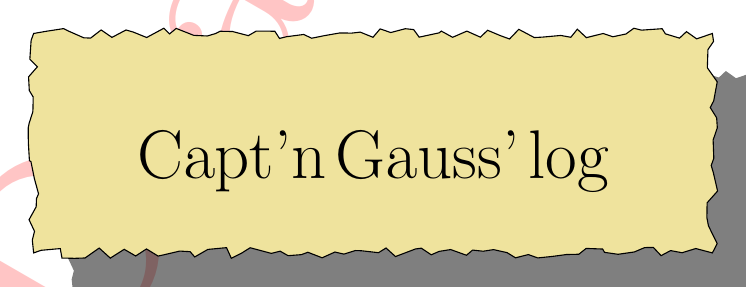
\begin{tikzpicture}[pencildraw/.style={ %
    decorate,
    decoration={random steps,segment length=4pt,amplitude=2pt}
    } %
]
\node[
preaction={fill=black,opacity=.5,transform canvas={xshift=.5cm,yshift=-.5cm}},
pencildraw,draw,fill=paper,text width=3in,inner sep=.5cm] 
{\begin{center}\Huge Capt'n Gauss' log \end{center}\vspace{.7cm} {\huge\context}};
\end{tikzpicture}}

\end{tabular*}

\vfill

\includegraphics[width=3in]{logoPirate.png}\hfill \includegraphics[width=2in]{bammLogo.png}


}


\begin{document}



\begin{context}
  Ahoy me Mathys! At ye port of Pythagoras, be a Pizzaira that will
  make a pizza with arrangements of toppings to befudle the mind.


  \vspace{1cm}

  
  Help me feed me crew, and I can help ye find me treasure!
\end{context}



\begin{directions}
  Apply toppings on the pizza so that
  \begin{itemize}
  \item Each pirate gets the same amount of pizza.
  \item Each pirate gets what they want
  \end{itemize}
\end{directions}



\begin{example}
  $1$ out of $3$ of my pirates want peppers

  $2$ out of $3$ want anchovies.


  How do I feed my crew of $12$?
\begin{center}
  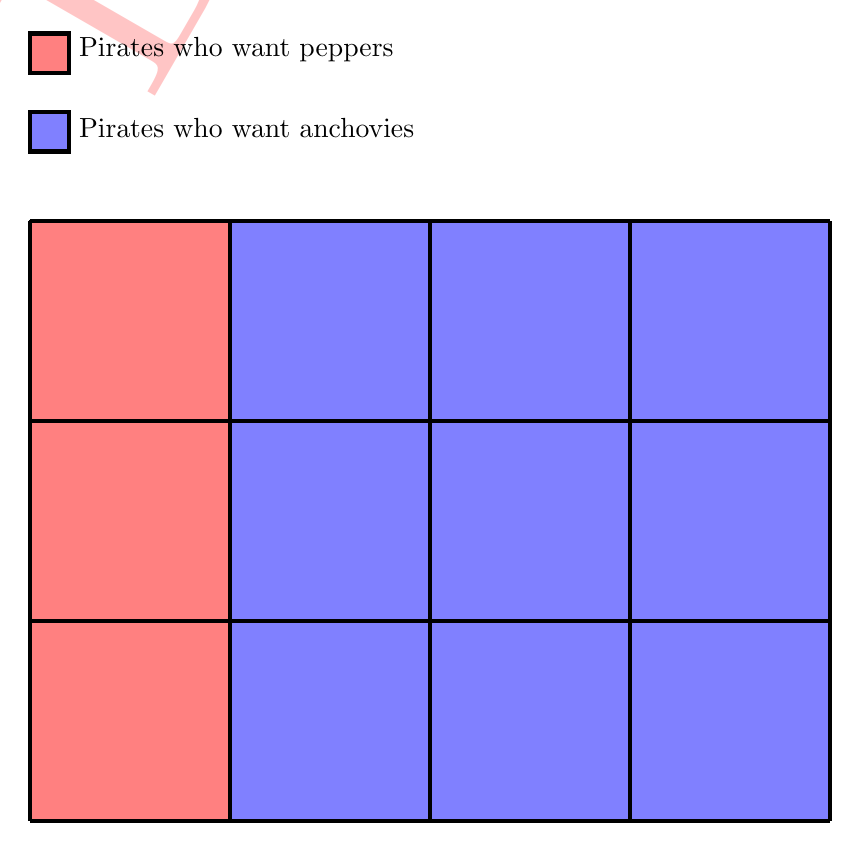
\begin{tikzpicture}
    \draw[fill=red!50!white,ultra thick] (0,9.5) rectangle (.5,10);
    \draw[fill=blue!50!white,ultra thick] (0,8.5) rectangle (.5,9);
    \node[right] at (.5,9.8) {Pirates who want peppers};
    \node[right] at (.5,8.8) {Pirates who want anchovies};

    \draw[fill=red!50!white] (0,0) rectangle (1in,3in);
    \draw[fill=blue!50!white] (1in,0) rectangle (4in,3in);
    \draw[step=1.0in,black,ultra thick] (0,0) grid (4in,3in);
    
\end{tikzpicture}
\end{center}
\end{example}



\begin{mathConnections}
  https://bartsnapp.github.io/Math-Outreach-Exhibits/pizza/pizza/
\end{mathConnections}
\end{document}
